% This is LLNCS.DEM the demonstration file of
% the LaTeX macro package from Springer-Verlag
% for Lecture Notes in Computer Science,
% version 2.4 for LaTeX2e as of 16. April 2010
%
\documentclass{llncs}
%

%\usepackage{makeidx}  % allows for index generation
\usepackage{cite}
\usepackage{color}
%\usepackage{balance} % Not needed for llncs
\usepackage{times}
\usepackage{url}
\urlstyle{same} % formats footnotes
\usepackage{xcolor}
\usepackage{pgfplots}
\usepackage{soul} % highlighting
%\usepackage{multirow}
\usetikzlibrary{patterns} %% Used for bar charts
\usepackage{float} %% Used for side by side minipages
\usepackage{multirow}
\usepackage{subfigure} % Needed for showing charts side by side

\usepackage{amssymb}% Checkmark



\newcommand{\todo}[1]{\textcolor{cyan}{\textbf{[#1]}}}
\newcommand{\dan}[1]{\textcolor{blue}{{\it [Dan says: #1]}}}
\newcommand{\andy}[1]{\textcolor{blue}{{\it [Andy says: #1]}}}
\newcommand{\sam}[1]{\textcolor{blue}{{\it [Sam says: #1]}}}

\begin{document}

% An

\title{An Empirical Analysis of Crash Dump Grouping}
\author{Daniel E. Krutz and Samuel Malachowsky}
\institute{Rochester Institute of Technology, Rochester NY 14623, USA \\
\email{\{dxkvse, samvse\}@rit.edu}
}



%\author{Daniel E. Krutz\inst{1} \and Wei Le\inst{2}}
%
%\institute{Rochester Institute of Technology, Rochester NY 14623, USA\\
%\email{dkrutz@se.edu}
%\and
%Iowa St. University, Ames, IA, 50011, USA\\
%\email{weile@iastate.edu}
%}

% %\affil[1]{Department of Software Engineering, Rochester Institute of Technology}

\maketitle

\begin{abstract}

Software developers are involved in a constant struggle to produce high quality software. Crash dumps are an important resource for gathering invaluable information about software defects in the field. The goal of this paper is to compare manually and automatically grouped crash dumps and discover grouping criteria that are effectively used in manual diagnosis. In our study, we compared a total of 1,550 groups and 30,431 crash dumps from 5 Mozilla applications. We found that 1) call stacks are more dissimilar from each other in manual groups, in addition to matching call stacks, developers frequently use multiple resources, such as reproduction steps and revision histories, for grouping crashes; 2) while automatic tools focus on grouping crashes based on the same root cause, developers also correlate crash dumps across different versions of programs or even different applications for related root causes; 3) both automatic and manual approaches are imprecise, but the two make different types of mistakes. From this study, we determined that to more effectively group crashes,  future tools should: 1) enable multiple criteria and explore diverse uses of crash dump groups for prioritizing and fixing bugs, 2) correlate multiple sources of information or even multiple applications, and 3) uncover inherent relations between symptoms and source code.

%%% Previous abstract. Shortened to save space
%Software developers are involved in a constant struggle to produce high quality software. Crash dumps are an important way that developers may gather invaluable information from software defects in the field. Each defect can be repeatedly triggered by different users, which will likely create an overwhelming number of crash dumps on a daily basis, which can create an vast amounts of data to examine, which makes crash grouping techniques of paramount importance. Unfortunately, crash grouping techniques often incorrectly group irrelevant crash dumps or miss related crash dumps which will then fail to provide developers the accurate information they require to fix the software's defect.
%
%The goal of this paper is to compare manually and automatically grouped crash dumps and discover grouping criteria that are effectively used in manual diagnosis, but lacking in automatic tools, from which we potentially enable more precise and capable crash diagnostic tools. In our study, we compared a total of 1,550 groups and 30,431 crash dumps from 5 Mozilla applications. We found that 1) call stacks are more dissimilar from each other in manual groups, as besides matching call stacks, developers frequently link multiple sources, such as reproduce steps and revision histories, for grouping crashes; 2) while automatic tools focus on grouping crashes based on the same root cause, developers also correlate crash dumps across different versions of programs or even different applications for related root causes; 3) both automatic and manual approaches are imprecise, but the two make different types of mistakes; and 4) for small applications, developers' domain knowledge on code works more effectively than the automatic approach for correlating crashes.  From this study, we determined that to more effectively group crashes,  future tools should 1) enable multiple criteria and explore diverse uses of crash dump groups for prioritizing and fixing bugs, 2) correlate multiple sources of information or even multiple applications, and 3) uncover inherent relations between symptoms and source code.


\keywords{Crash Dumps, Call Stacks, Grouping, Similarity}


\end{abstract}


%%% Make sure to tell the "Story" of the work we are hoping to accomplish.
\section{Introduction}~\label{sec:intro}
Due to the complexity of applications, it is impractical to expect perfect software on the initial release. Thus, an important and challenging task during software maintenance is to capture and diagnose failures triggered at the client side. Examples of such feedback systems include Microsoft's Dr. Watson~\cite{watson} and Mozilla Crash Reporter~\cite{mozilla}. In these systems, crash dumps which typically contain call stacks recorded at the crash site, are used for locating bugs in software. Since the same bug can be repeatedly triggered by different users and under different execution environments, the number of crash dumps submitted daily can reach millions~\cite{firefox}. Incorrectly grouping unrelated crash dumps or failing in identifying a new crash that actually belongs to an already fixed group can incur unacceptable manual overhead and potentially delay critical patches. Thus, it is imperative to find effective criteria for precisely correlating crash dumps, from which we can use to develop fast and automatic tools.

Grouping crash dumps is challenging because the dumps primarily contain information that indicates dynamic symptoms of a bug, such as call stacks and register values. However, to locate a root cause and introduce a fix, we need to identify the part of the source code that is responsible for the crash. Since the same symptoms are potentially caused by different pieces of wrong code or the same piece of problematic code can result in completely different call stacks at the crash, techniques purely based on dynamic symptoms for grouping crashes are insufficient~\cite{Bartz:2008:FSF:1855895.1855896,brodie:automated,4401026,Kim:2011:2}.

The goal of this work is to discover criteria and methodologies that are effectively applied in manual diagnosis for grouping crash dumps but lacking in automatic tools; from these, we aim to derive guidelines for designing new and more effective crash diagnostic tools. Specifically, our objectives are to determine 1) beyond the traditional criterion of grouping crash dumps based on the same root cause, whether we can find more types of connections between crash dumps; and 2) to determine what sources of information should be used beyond call stacks.

We performed a comprehensive comparison on {\it m-groups}: manually grouped crash dumps, and {\it a-groups}: automatically grouped crash dumps. Our dataset consists of a total of 1,550 groups and 30,431 individual call stacks from 5 Mozilla applications. For m-groups, we extract crash dumps from Bugzilla entries that are confirmed as {\it related} by developers. For {\it a-groups}, we chose groups automatically generated by Mozilla Crash Reporter~\cite{mozilla}. Similar to most automatic tools~\cite{Bartz:2008:FSF:1855895.1855896,brodie:automated,4401026}, Mozilla Crash Reporter uses call stack information to determine crash dump groups. These crash dumps are reported from deployed, mature applications such as Firefox and Thunderbird~\cite{firefox}.

%%% Removed to save space
%\begin{table*}
%\centering
%\caption{Summary of our Findings\label{tab:findings}}
%\resizebox{\textwidth}{!}{
%\begin{tabular}{|l|l|l|l|l|}\hline
%Research Questions&Comparison Metric&Automatic&Manual&Implications\\\hline\hline
%\multirow{2}{*}{Why we group crashes}&\multirow{2}{*}{Grouping criteria}&Single:&Multiple:&Exploit the uses of groups to\\
%&&same cause&same, related causes, who should fix&better prioritize and fix bugs\\\hline
%\multirow{4}{*}{How we group them}&\multirow{2}{*}{Grouping info}&Limited:&Multi-sources:&Correlate multi-sources info,\\
%&&signatures, call stacks&black-box + white-box info&multi-versions, multi-applications\\\cline{2-5}
%&\multirow{2}{*}{Imprecision}&Fundamental:&Ad-hoc:&Design better tools to reveal\\
%&&based on symptoms&incorrectly parse and link info&relations between symptoms and code\\\hline
%\multirow{2}{*}{What are the capabilities}&Call stack&Scalable:&Diverse:&Grouping based on call stacks is \\
%&characteristics&larger, more call stacks&dissimilar between call stacks&insufficient, especially for small apps\\\hline
%\end{tabular}
%}
%\end{table*}


For comparing a-groups and m-groups, we define four metrics: 1) what criteria are chosen to correlate the crash dumps? 2) what information is used to derive the groups? 3) is there any imprecision related to the grouping and why? and 4) what are the characteristics of call stacks in a-groups and m-groups? To answer these questions, we analyzed developer discussion logs on the 452 Bugzilla entries. These entries display the diagnostic process developers perform to correlate crash dumps from Bugzilla entries as well as ones from Mozilla Crash Reporter. To conduct the comparisons on (4) above, we automatically compute the sizes of grouped call stacks and also similarity measures between call stacks such as Brodie metrics~\cite{brodie:quickly} and longest common substrings. We found that:

%%% Removed to save space
%The contributions of our paper are summarized in Table~\ref{tab:findings}. The first column lists the research questions we aim to explore. The second column summarizes a set of comparison metrics we define for answering the research questions. Under {\it Automatic} and {\it Manual}, we list a set of observations discovered from analyzing a-groups and m-groups. Under {\it Implications}, we provide our insights on how to design effective crash diagnostic tools learned from the study.


\begin{enumerate}
\item Developers correlate crash dumps not only for the shared root causes, but also for the related causes and for who can fix them. Diagnosis based on a group of crash dumps is sometimes more informative than diagnosis based on a single crash dump.
\item Developers coordinate multiple sources of information, multiple versions of programs and sometimes different applications to determine the groups, which enables many dissimilar call stacks to be correctly grouped.
\item Mistakes in grouping crash dumps could take months to be corrected. Automatic approaches based on dynamic symptoms are fundamentally imprecise, while developers make ad-hoc mistakes. An effective tool should establish precise relations between symptoms and code.
%\item Automatic approach is scalable; however, manual diagnosis is more effective in grouping crash dumps in small applications.
\end{enumerate}


This paper is organized as follows: Section~\ref{sec:approach} explains how we collect the dataset and perform the study. Section~\ref{sec:results} presents our comparison results analyzed from 5 Mozilla applications. In Section~\ref{sec:related}, we summarize the related work, and in Section~\ref{sec:limitations}, we discuss the limitations of our study. Section~\ref{sec:conclusions} concludes our work.

\section{Dataset and Methodologies}~\label{sec:approach}
In this section, we present how our dataset is constructed and how the information regarding a-groups and m-groups is collected for comparison.

\subsection{Data Collection Process}
%% Look at feedback asking for elaboration on the data collection process
%%% GC Scraper: https://code.google.com/p/dk-crashsignature/
In order to collect the necessary data for our study, we built a collection and analysis tool called Mozilla Call Stack Grouper (MCSG) which consisted of several stages. The initial step of MCSG is the data collection phase where the user first selects a group of crash stacks to be analyzed, which may be for a specific Mozilla application and version. For example, the user may choose to analyze all call stacks for Mozilla  Firefox 46.0a1. MCSG will then pull the \emph{top crasher} call stacks for the specified application and version from the Crash Stats Mozilla website\footnote{https://crash-stats.mozilla.com/}. A \emph{top crasher} is a crash type with one of the highest number of crash reports on the Mozilla website~\cite{Dhaliwal:2011:CFC:2117694.2119726}. % Is this citation needed?


% Make sure that all three of these measurement mechanisms are actually used
The data collection process begins by gathering the call stacks and developer discussion logs for these top crashers, which is done using HttpUnit\footnote{http://httpunit.sourceforge.net}. Each of the collected call stacks are stored locally in a .txt file in the folder with all the other call stacks from the same top crasher group. Once all of the folders and call stacks have been collected, the comparison process may begin. There are several existing techniques for measuring call stack similarity~\cite{Bartz:2008:FSF:1855895.1855896, 4401026}. MCSG measures call stack similarity using the call stack similarity metrics as defined in these works. %If a researcher wishes to add, modify or remove a call stack similarity measurements algorithm to the tool, it is designed to make this as easy as possible.

Some of the primary challenges which needed to be overcome in the creation of MCSG was the ability to accurately collect the necessary information, especially with the format of the crash source frequently changing.  A second significant problem to be overcome was the implementation of the crash comparison mechanisms. While the implementation of the comparison algorithms was a fairly straightforward task, the number of comparisons and evaluations which needed to be completed was very large, and therefore creating an analysis mechanism which would operate accurately and efficiently was a challenging task. We spent a large amount of time optimizing our comparison algorithm and verifying its accuracy.


%This custom built scraper and collected data is further discussed in Section~\ref{sec:publicdata}.

%%% Give a number of the comparisins?

%%%%

%In order to collect the necessary data for our study, we built a custom scraper tool which consisted of several stages. The initial phase used pulled the necessary crash information from each of the Mozilla crash information websites. Using HttpUnit\footnote{\url{http://httpunit.sourceforge.net}} as a foundation, the tool collected the crash stacks, the crash's signature name\todo{.....},  \todo{make sure all the information is included here}. Once the information was gathered, a second component of the tool analyzed

% Primary challenges to overcome - maybe put into the tools section ?

%%% Make sure this is being added in the appropriate spot and that it is also not located someplace else in the paper
%\todo{Proofread all of this}
%\todo{developer discussion logs?}

% \ti - Dont know what this is

%%% crashes were collected as .txt files

\subsection{Dataset: a-groups and m-groups}
When a crash occurs at the client side, a {\it crash dump} is generated by the deployed crash management system. Typically, it captures the program state at the crash as well as static information about the system and software. For example, a crash dump returned by Mozilla Crash Reporter(MCR) primarily includes: 1) call stacks of each active thread at the crash, 2) exception types captured at the crash such as EXCEPTION\_ACCESS\_VIOLATION\_WRITE, and 3) operating system, software and their versions, as well as the building, installation and crashing dates and time.  When a user clicks the {\it submit crash report} button, the crash dumps are sent back to the server for postmortem analysis.

MCR organizes groups of crash dumps based on applications. For each application, it ranks most frequently occurred crash dump groups within a certain time window. A user can also send in crash information manually through Bugzilla~\cite{bugzilla}, in which case, the crash information is constructed in ad-hoc based on the users' judgment. Compared to crash dumps generated automatically, the report in Bugzilla may contain additional information, such as 1) reproduce steps that lead to crashes, 2) code segment that is suspected to cause the crash, 3) the URL visited when the application crashes, 4) expected results, 5) the other bugs that may be relevant, and 6) any connections to groups of crash dumps reported by Mozilla Crash Reporter.

Figure~\ref{fig:dataprocess} demonstrates how a-groups and m-groups in our study are constructed. The groups of crash dumps are selected from both Mozilla Crash Reporter and Bugzilla across five applications including {\it Firefox}, {\it Thunderbird}, {\it Fennec}, {\it FennecAndroid} and {\it SeaMonkey}. For a-groups, we collected maximally 300 top crash dump groups for each application. For m-groups, we inspect the summary page Mozilla presents for each a-group, shown in Figure~\ref{fig:bugzilla}. From this page, we find Bugzilla entries that are correlated to the a-group, shown in Figure~\ref{fig:bugzilla}. We recursively search each correlated Bugzilla entry to find more Bugzilla entries that are confirmed to be relevant. The crash dumps reported in these Bugzilla entries constitute an m-group. As an example, in Figure~\ref{fig:dataprocess}, $b_1$ and $b_2$ are the two Bugzilla entries found relevant to {\it a-group} and $b_3$ is identified by recursively inspecting $b_1$ and $b_2$ for related bugs. The Bugzilla entries also contain developer discussions on how to diagnose the crash dumps.


%%%%% Did not use since I had a had time getting both to fit well side by side
%\begin{table}[t]
%\begin{minipage}[b]{.50\textwidth }%
%
%\includegraphics[scale=0.45]{images/approach1.png}
%
%\end{minipage}%
%\begin{minipage}[b]{.45\textwidth}
%\centering
%
%\includegraphics[scale=0.45]{images/bugzilla.png}
%
%\hrule height 0pt
%\end{minipage}
%\end{table}


\begin{figure}[!htb]
\centering
%\includegraphics[width = 8.4cm, angle = 0]{approach1.ps}
\includegraphics[width = 8.4cm, angle = 0]{images/approach1.png}
\caption{\small Collect a-Groups and m-Groups~\label{fig:dataprocess}}
\normalsize
\end{figure}

\begin{figure}[!htb]
\centering
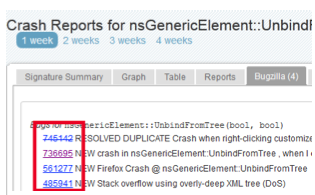
\includegraphics[scale=0.8]{images/bugzilla_updated.png}
%\includegraphics[width = 5.4cm, angle = 0]{images/bugzilla.png}
%\includegraphics[width = 5.4cm, angle = 0]{bugzilla.ps}
\caption{Link a-group and m-group~\label{fig:bugzilla}}
\normalsize
\end{figure}

\begin{table}
\caption{Dataset from 5 Mozilla Applications\label{tab:dataset}}
%\resizebox{\columnwidth}{!}{
\center
\begin{tabular}{|l||c|c||c|c|c|}\hline

\multirow{2}{*}{Program} & \multicolumn{2}{|c||}{a-Groups} & \multicolumn{3}{|c|}{m-Groups} \\\cline{2-6}

&T$_g$&T$_c$&T$_g$&T$_b$&T$_c$ \\ \hline\hline

  Firefox &298&18316&20&110&233\\ \hline
  Thunderbird &299&3151&20&106&237\\ \hline
  Fennec &299&2567&20&87&155\\ \hline
  Fennec Android &297&4925&20&90&189\\ \hline
  SeaMonkey & 257&514&20&59&144\\ \hline

%Firefox 14.0a1&299&18316&1&16/8645&1743&12&20&110&233&3&39&&61\\ \hline
%Thunderbird 10.0&299&3151&16&16/355&1792&32&20&106&237&3&33&1024&93\\ \hline
%Fennec 2.1.2&299&2567&1&16/2233&1792&2&20&87&155&3&24&1456&46\\ \hline
%Fennec Android 13.0a1&168&4925&1&16/993&1165&2&20&90&189&3&24&1456&82\\ \hline
%SeaMonkey 2.7.2&257&514&1&15/15&196&5&20&59&144&3&16&596&6\\ \hline

\end{tabular}
%}
\end{table}

Table~\ref{tab:dataset} summarizes the dataset we collected. Under {\it T$_g$}, we display the number of a-groups and m-groups studied for each application. The first four applications contain more than 300 a-groups and by setting a threshold 300, we successfully collected 297 to 299 a-groups. For each application, we randomly select 20 a-groups, based on which we construct m-groups, as explained in Figure~\ref{fig:dataprocess}. Under {\it T$_b$}, we count the total number of Bugzilla entries associated with the 20 m-groups. In each Bugzilla entry, users can report multiple crash dumps related to the bug. Under {\it T$_c$}, we list the total number of crash dumps in the m-groups.

%%The data indicate that on average, each Bugzilla entries contain 2--3 crash dumps. %%% DK: 2/17/16: I don't think this last sentence made much sense.


\subsection{Comparison Metrics and Approaches}
Using our dataset of a-groups and m-groups, our goal is to determine whether manual and automatic approaches apply consistent criteria and information to group crashes, and whether the two approaches correlate same types of call stacks. As shown in Figure~\ref{fig:approach}, we compare the groups based on the four metrics, including:
\begin{itemize}
\item {\it Grouping criteria}: How can we group crash dumps and how the groups can be used?
\item {\it Grouping information}: What information shall we use, and how shall we use it, for more effectively grouping crash dumps?
\item {\it Imprecision in the groups}: When do we group unrelated crash dumps or when do we fail to find the relevant crash dumps?
\item {\it Characteristics of call stacks}: What are the patterns in call stacks in a-groups and m-groups? How do the characteristics imply the capabilities of the two approaches?
\end{itemize}


\begin{figure}[!htb]
\centering
\includegraphics[width = 8.4cm, angle = 0]{images/approach2.png}
%\includegraphics[width = 8.4cm, angle = 0]{approach2.ps}
\caption{Compare a-Groups and m-Groups~\label{fig:approach}}
\normalsize
\end{figure}


The following steps are used to collect information for performing comparisons:

% How were the keywords developed
% Why were these a good idea to use
%

{\bf Identifying grouping criteria and information.} For a-groups, we studied documentation related to Mozilla Crash Reporter to understand the criteria and algorithms used. To determine grouping criteria and information used for m-groups, we analyzed  452 Bugzilla entries where the m-groups are determined. For learning grouping criteria, our focus is to determine what relations are established between crash dumps in the group and how developers compare and contrast crash dumps in a group for prioritizing, diagnosing and fixing the code. To obtain information important for correlating crash dumps, we defined a set of keywords, representing potential sources of information,  e.g., {\it call stacks}, {\it reproduce steps}, {\it regression windows}, {\it URL}, {\it plugin} and {\it libraries}. These keywords were chosen due to our observed frequency in crash data. Based on these keywords, we extract relevant text from the Bugzilla entries. We then count the frequencies at which each type of information is used and also the frequencies at which different types of information are combined in determining a group.


% How do we know that the process of how we justify imprecision was good & accurate?
%

{\bf Determining imprecision in a-groups and m-groups.} In this step, we aim to learn the existence, causes and consequences of imprecision for both of the approaches. To determine imprecision in a-groups, we randomly selected 100 a-groups from our dataset and for each a-group, we analyze the relevant Bugzilla entries that contain diagnostic information for the a-groups. We determine an a-group is imprecise if the developers confirm that the a-group: 1) contains a corrupted signature or call stack, 2) includes crash dumps that should not be correlated, and 3) fails to group crash dumps that should be correlated. Imprecision in m-groups is caused by developer error. We inspect developer discussion logs in the Bugzilla entries and identify cases where developers believe unrelated crash dumps are grouped by mistakes.

%% How is this information beneficial?
%% What do we hope to learn from this information

{\bf Comparing call stack characteristics.} To compare the capabilities of manual and automatic approaches, we study the patterns in call stacks for a-groups and m-groups. To determine if there is a pattern, we also construct {\it r-groups}; each of the r-groups contains the random number of crash dumps randomly selected from a-groups. We compare a-groups and m-groups regarding 1) the sizes of groups, including the number of call stacks in each group and the length of the call stacks, and 2) the similarity between call stacks. We compute the metrics in string matching algorithms to measure the similarity between the call stacks, including the {\it Brodie value} ({\it B-Value}), {\it Brodie weight} ({\it B-Weight})~\cite{brodie:automated,brodie:quickly}, longest common substrings ({\it LCS}), and the percentage of identical call stacks in a group ({\it C-Identical}). In the following, we explain how each of the measure is calculated. Suppose $m$ is the number of {\it matching lines} between two call stacks, and $l_1$ and $l_2$ are the lengths of the two call stacks. Brodie value $bv$ is computed as:

\[
  bv = \left\{
  \begin{array}{l l}
    m/l_1 & \quad l_1 == l_2\\
    m/((l_1+l_2)/2) & \quad l_1\neq l_2\\
  \end{array} \right.
\]

We consider a {\it matching line} between two call stacks if at location $i$ from the top of the call stacks $C_1$ and $C_2$, the function names $C_1[i]$ and $C_2[i]$ are identical. Brodie weight is a string similarity metric improved from the Brodie value. It distinguishes the weight of the functions in call stacks for determining similarity. The assumption is that functions located at the top of the call stack should have more weight than ones located at the bottom. The detailed algorithm of how to compute Brodie weight between two call stacks is given in~\cite{brodie:automated}.

%\IncMargin{1em}
%\LinesNumbered
%\begin{algorithm}[!htb]
%\SetFuncSty{bf}
%\SetKwData{ans}{Unsolved}
%\SetKwFunction{icfg}{BuildICFG}
%\SetKwInOut{Input}{Input}
%\SetKwInOut{Output}{Output}

%\Input{Specification of Fault, $spec$}
%\Output{Calls to {\bf MatchFSignature}, {\bf MatchDSignature};\\

%A repository of function definitions, $R$}
%\BlankLine

%\caption{Generating Analysis\label{alg:generation}} %{\bf MatchFSignature} and {\bf MatchDSignature}
%\normalsize
%\end{algorithm}

We obtain the Brodie value/weight for a group by adding up the Brodie value/weight for every two call stacks in the group and then dividing the times of comparisons. Finally, we get an average across groups for an application. To compute LCS across all the call stacks in a group, we first detect a set of common substrings between two call stacks. We then determine whether other call stacks in the group contain the same common substrings. The comparison is performed between the average LCS across a-groups and the average LCS across m-groups for an application. The {\it C-Identical} identifies the maximum number of crash dumps in a group that are actually identical, calculated by $n_i$/$n$. In an a-group or m-group, we may find several subgroups, within which, crash dumps are identical. $n_i$ here is the number of identical call stacks in the largest subgroup and $n$ is the size of the a-group or m-group.

\section{Results}~\label{sec:results}
In this section, we present our comparison results and our insights for designing better grouping tools.

\subsection{Comparison based on Grouping Criteria}



\textbf{RQ1: How can we group crash dumps?}


%\todo{reorder - present data 1st and then develop big picture}




%%%% I think this should be left out as it does not appear to have been included in the 2012 submission
%\begin{figure}
%\begin{minipage}[b]{\textwidth}
%\centering
%\includegraphics[width = \columnwidth, angle = 0]{group.ps}
%\end{minipage}
%\caption{Fault Localization Based On Call Stacks~\label{fig:group}}
%\end{figure}

Our first research question was how crash dumps are grouped to associate related crashes with one another. For automatic approaches that compare call stack similarity for grouping crash dumps, the implied grouping criterion is that the crash dumps in a group should share the root cause. However, we find that the grouping criteria applied in manual diagnosis are more diverse and flexible. In Table~\ref{tab:goal}, we summarize our discoveries. Similar to automatic approaches, in many cases, developers correlate crash dumps if they believe these crashes are originated from the same bug in the code. In another word, if we introduce a fix based on any crash in the group, we can fix all the crash dumps grouped, and if a new crash dump is determined to belong to the group, we do not need to further diagnose it.

\begin{table}[!htb]
\centering
\caption{Grouping Criteria for m-Groups\label{tab:goal}}
%\resizebox{\columnwidth}{!}{
\begin{tabular}{|l||l|l|}\hline
Grouping Criteria&Goals\\\hline\hline
\multirow{4}{*}{Same Root Cause}&Fix one to fix all in the group\\\cline{2-2}
&Determine if a given new crash is fixed\\\cline{2-2}
&Localize bugs via comparing similar stacks\\\cline{2-2}
&Learn bug manifestation to prioritize them\\\hline\hline
\multirow{2}{*}{Related Root Cause}&Localize root causes if fix to previous\\
&crashes is the cause for the current crash\\\hline\hline
\multirow{2}{*}{Who Fixed the Bug}&Find experts who can fix a group of bugs\\
&from the same code region or of same types\\\hline
\end{tabular}
%} % resize box
\end{table}


Interestingly, although the goal of grouping crash dumps is to avoid repeatedly diagnosing crash dumps caused by the same root cause, developers still frequently compare multiple crash dumps in the same group for determining the types and locations of a bug. This indicates that a group of crash dumps can be more informative than individual crash dumps in helping diagnose failures. For example, a same bug may cause completely different symptoms, and we find a case where developers prioritize a group of crash dumps because one of the crashes have the serve symptom related to a security attack. As shown in the Table~\ref{tab:goal}, developers also correlate crash dumps if the root causes that lead to the crashes have a temporal or locality relationship.

In our study, we find cases where one crash is caused by an incomplete/incorrect fix to the other crashes. Developers believe that correlating these crashes can help quickly identify the cause and the fix for the newly generated crashes. The components where the crashes occur, together with the bug types, are used to determine the groups. The goal is to better distribute the debugging tasks to people who are most familiar with the code and the bug types.

%Thus, to summarize the findings of our research question we found that:
In summary to our research question about crash dump grouping, we found that:

\begin{enumerate}
\item Besides grouped based on the same root cause, crash dumps can also be correlated if the patch to one crash is the cause for another crash.
%% Removed for SEFM \item Developers also group crash dumps if they can be conveniently fixed together, for example, by a same developer.
\item Diagnosing a group of crash dumps can be beneficial: first, a group of symptoms help determine general manifestation of a bug; second, a group of similar call stacks potentially enable automatic bug localizations.
\end{enumerate}





%\noindent
%\textbf{Analysis}
%\todo{Provide more of an analysis of things here.....}
%% What are some actionable results of things



\subsection{Comparison based on Grouping Information}

\textbf{RQ2: What information shall we use to group crashes?}


%\todo{reorder - present data 1st and then develop big picture}

We next sought to determine the best information to effectively and efficiently group crashes. Mozilla Crash Reporter automatically groups crash dumps by matching 1) the version of software where the crash dumps are originated; and 2) the function call on the top of the call stack at the crash, called {\it signature}. On the contrary, developers use a variety of information. No systematic way is applied to choose which source of information should be used for determining a particular group of crash dumps. %%%% Fix this sentence?

\begin{figure*}
%\begin{minipage}[b]{\textwidth}
%\subfigure[Same Signature, Different Causes]{
\scalebox{.8}{
\subfigure[List of Information Source]{
\includegraphics[width = 6.6 cm, angle = 0]{images/Info1.png}
% \includegraphics[width = 6.6 cm, angle = 0]{Info1.ps}
~\label{fig:ind}
}
\subfigure[Linking Multiple Sources]{
\includegraphics[width = 9.0 cm, angle = 0]{images/Info2.png}
% \includegraphics[width = 9.0 cm, angle = 0]{Info2.ps}
~\label{fig:multi}
}
} % scale
%\end{minipage}
\caption{Information Used for Manually Grouping Crash Dumps~\label{fig:stack}}

\end{figure*}

We studied a total of 40 m-groups from Firefox and Thunderbird and found that developers generally apply three types of information for grouping crash dumps: 1) white-box information, i.e., crash symptoms related to code including call stacks and their signatures, 2) black-box testing information, e.g. steps on triggering the bug, and 3) information related to software versions, such as build time and revision histories. We summarize our analysis results in Figure~\ref{fig:stack}. On the left, we rank a list of information source developers frequently use in determining crash dump groups, and on the right we show the correlation of these sources applied in manual diagnosis. The $y$-axis presents the percentage of crash dumps that are grouped using the specific source(s) of information.

In Figure~\ref{fig:ind} the $x$-axis, {\it Stack} represents call stacks. {\it Env} indicates the plugins and libraries involved in the crash. {\it Correlation}, used by Mozilla Crash Reporter, specifies how often a signature and a .dll component are simultaneously witnessed in a crash. For example, given a set of call stacks, we count that a certain signature occurs 10 times, and among the 5 times, a specific .dll also occurs; in this case, the correlation ratio between the signature and the component is 50\%. {\it Repro} and {\it URL} indicate two relevant types of testing information. {\it Repro} represents the steps taken to reproduce the bug and {\it URL} refers to a list of URL visited before an application crashes. {\it Revision} is a list of changes made to the application shortly before a crash. Finally, {\it Build} gives the date and time to indicate when the application is built and installed, as well as the version of operating system where the application runs.

Figure~\ref{fig:ind} shows that call stack, build information and reproduction steps are the three most frequently used sources. For Firefox, 67\% of the crash dumps were grouped using call stacks, 26.4\% applied build information and 24.5\% were determined using reproduce steps. Similarly, for Thunderbird, 62.7\% used call stacks,  38.2\% used the build information and 37.3\% applied reproduce steps. The secondary important source is {\it Revision}, based on which, 8.5\% of the Firefox crash dumps and 9.1\% of the Thunderbird crash dumps are grouped. By inspecting m-groups determined using {\it Revision} information, we find that when crashes occur shortly after a new release of an application, plugin or operating system, developers give the priority to consider whether the crash dumps can be caused by the same bug in the new code and thus can be grouped together. Sometimes, the developers suspect that the crash dumps are caused by bugs in a certain plugin or operating system, and thus they correlate crash dumps from different applications running with the same plugin or operating system.

% developers would determine if a particular type of crash dumps only occur after new releases of applications, plugins or even operating systems. Consider the number of bugs in new code may be small, the crash dumps are likely to be caused by the same bug in the new code and thus can be grouped together. If developers suspect the crash dumps are related to plugin or OS, they link crash dumps from multiple applications.

 %It is useful in determining if, and what recent alterations may have caused the crash. If a previous patch would have fixed or caused the issue. This is the same as looking to see if a previous build of the application could have caused the issue, or if it is used to find correlations between bugs.  If the occurrence of the crash is correlated to a major release with operating systems such as Windows patches, crash dumps occurred at the similar time, will be attributed to as likely due to a bug in new release code. Sometimes they will group crash dumps from multiple applications that run in the same environments.

In Figure~\ref{fig:multi}, we show that developers often make decisions by coordinating multiple sources of information. The left bars in the figure indicate that 70\% of the crash dumps from Firefox and 68.8\% from Thunderbird are grouped by using more than one source of information. Consistent with Figure~\ref{fig:ind}, developers most frequently link call stacks, build information and reproduce steps to determine the groups. As shown in Figure~\ref{fig:multi}, the top three combined sources include 1) call stack with build information, 2) call stack with reproduce steps and 3) reproduce steps with build information. Correlating Figure~\ref{fig:ind} and~\ref{fig:multi}, demonstrates interesting findings. For example, we can derive that 67\% of the Firefox crash dumps are grouped using call stacks.

%%% Was confusing.
%\hl{For example, we can derive that 67\% of the Firefox crash dumps are grouped using call stacks, among which about a half are used with the reproduce steps and half are used with build information. The three of the sources might be used together in some cases.}

Our inspection in m-groups shows that developers often use build information as the first step to reduce the scope of the grouping. However, grouping crash dumps of the same version is often not ideal because different versions of a program may contain the same problematic code and any crash dumps caused by this code should be grouped. We also discover that coordinating call stacks and reproduce steps can be challenging. We found a case where developers compare a crash dump with call stacks in non-crash threads to determine what steps in testing can produce a specific sequence of calls in the call stacks.

In summary to our research question about the information used to group crashes, we found that:

\begin{enumerate}
\item Call stacks, build information and reproduce steps are the three main sources for developers to group crashes.
\item Developers frequently correlate multiple sources of information for determining the groups. For example, developers once linked call stacks and reproduce steps by comparing call stacks in crash dumps with the call stack in a non-crash thread.
\item Developers correlate crash dumps across applications to determine if the root cause is located in the shared libraries or plugins.
\item Different versions of programs can contain the same piece of problematic code, and thus we should enable the grouping across different versions of the code.
\end{enumerate}

%The build information helps determine which version of code the crash is originated. The rationale is that crash dumps in a group 1) could origniate from different versions of code, but all of which should contain a same bug 2) manifest similarity in call stacks and/or 3) crash dumps can be reproduced following the similar steps. Automatic approach groups stack only based on the same version of code can miss related crash dumps. We need to find a way to correlate call stacks and reproduce steps.



%\noindent
%\textbf{Analysis}
%\todo{Provide more of an analysis of things here.....}
%% What are some actionable results of things

\subsection{Comparison based on Imprecision}

\textbf{RQ3: When do we group unrelated crash dumps and when do we fail to find the relevant crash dumps?}

For our third research question, we analyzed common mistakes in crash dump grouping. We first show our results on imprecision in m-groups. In Table~\ref{tab:mistake}, we list the four examples confirmed as developer mistakes. Under {\it Bug ID}, we list the identifications of the Bugzilla entries where the mistakes are found. Under {\it Developer Mistakes}, we give the descriptions of the mistakes. Under {\it Time}, we show the time period from when the mistake is firstly introduced to the Bugzilla post to when the developers confirm the problems. In the first two cases, developers misread the call stacks and mismatched the code. In the third case, developers only used signatures, the approach implemented in Mozilla Crash Reporter, rather than performed a more depth analysis to determine the group. In the fourth case, developers made a wrong judgment and believed the crash is a regression of a previous a bug. The results show that these mistakes can be difficult to discover, and the time that takes to find the problems is not always proportional to the complexity of the mistake. The implication of this result is that we need to develop automatic tools to help avoid these simple but expensive mistakes from developers.
\begin{table}[!htb]
\centering
\caption{Imprecision in m-Groups: Example Mistakes\label{tab:mistake}}
%\resizebox{\columnwidth}{!}{
\begin{tabular}{|c||l|l|}\hline
Bug ID&Developer Mistakes&Time\\\hline\hline
716232&Mismatch call stacks&4.6 hours\\\hline
695505&Inspect wrong version of code&3.0 months\\\hline
524921&Match signature only&2.7 days \\\hline
703133&Incorrectly link to a patch& 4.7 days\\\hline
\end{tabular}
%} % resize box
\end{table}

\begin{table}[!htb]
\centering
\caption{Imprecision in a-Groups\label{tab:agroup}}
%\resizebox{\columnwidth}{!}{
\begin{tabular}{|c||c|c|c|}\hline
Total&Corrupted Stack&Group Unrelated& Fail to Group Related\\\hline\hline
100&4&2&4\\\hline
\end{tabular}
%} % resize box

\end{table}

In Table~\ref{tab:agroup}, we present the set of data that demonstrate the imprecision in a-groups. Our approach is to inspect the Bugzilla entries that document the manual diagnosis for the a-groups and find imprecision in a-groups confirmed by developers. Under {\it Total}, we show that we studied the Bugzilla entries related to a total of 100 a-groups in our dataset. Under {\it Corrupted Stack}, {\it Group Unrelated}, and {\it Fail to Group Related}, we list the number of instances for the three types of imprecision: 1) call stacks are corrupted at the crash and thus the signature returned is no longer the top function where the actual failure occurs; 2) crash dumps grouped in an a-group are actually irrelevant; and 3) crash dumps of the same/related root causes are not grouped in the same a-group.

In our study, we find that all three types of imprecision exist in a-groups. The actual instances may even be higher than the ones listed in the table, as developers may only discover a small portion of such problems. In the following, we present two examples discovered during inspecting these mistakes. The examples indicate that it is neither sound nor complete to group crash dumps based only on the equivalence of the signatures or the similarity of the call stacks. In Figure~\ref{fig:group2}, the two crash dumps are generated from the same cause in the same version of the program. However, because the crashes are triggered in different versions of Windows, the crash dumps contain different signatures (see the first row in the table) and thus were not grouped by Mozilla Crash Reporter.

\begin{figure}
\centering
%\resizebox{\columnwidth}{!}{
\begin{tabular}{|l|l||c|}\hline
Call Stack 1 & Call Stack 2 & Match\\\hline\hline
\multirow{2}{*}{\_SEH\_prolog}& InternalCallWinProc &\multirow{2}{*}{$\times$} \\\cline{2-2}
&UserCallWinProcCheckWow &    \\\hline
CallWindowProcAorW & CallWindowProcAorW & $\checkmark$\\\hline
CallWindowProcW  & CallWindowProcW & $\checkmark$\\\hline
mozilla::plugins::PluginInstance&mozilla::plugins::PluginInstance&\multirow{2}{*}{$\checkmark$}\\
Child::PluginWindowProc & Child::PluginWindowProc &  \\\hline
InternalCallWinProc &InternalCallWinProc  & $\checkmark$ \\\hline
%js::mjit::Compiler::checkAnalysis &js::mjit::Compiler::checkAnalysis &js::analyze::ScriptAnalysis::analyzeTypes \\\hline
\end{tabular}
%} % resize box
\caption{Same Cause, under Different Versions of OS, result in Different Signatures~\label{fig:group2}}
\end{figure}

In Figure~\ref{fig:stack2}, we show that by only comparing the similarity between call stacks, we can fail to distinguish a legitimate and illegal correlation between the call stacks. On the left in Figure~\ref{fig:stack2}, the two call stacks have the same signatures and 19 out of 26 calls in the first call stack have appeared in the second call stack. On the right of the figure, the two call stacks also contain the same signatures; however, only 10 out of 30 calls in the first call stack have appeared in the second. In fact, developers confirm that the first pair have irrelevant root causes, while the second pair should be correlated.  Any techniques using call stack similarity for grouping crash dumps could fail to correctly group the call stacks in the two cases.


\begin{figure*}
%\resizebox{\textwidth}{!}{
\subfigure{
\begin{tabular}{|l|l||c|}\hline
\multicolumn{3}{|c|}{Match 19/26, Different Causes }\\\hline\hline
js\_DestroyScriptsToGC&js\_DestroyScriptsToGC&$\checkmark$\\\hline
thread\_purger&PurgeThreadData&$\times$\\\hline
...&...&...\\\hline
XRE\_main&XRE\_main&$\checkmark$\\\hline
main&CloseHandle&$\checkmark$\\\hline
\end{tabular}
%} % resize box
\subfigure{
\begin{tabular}{|l|l||c|}\hline
\multicolumn{3}{|c|}{Match 10/30, Same Causes}\\\hline\hline
JSObject::nativeSearch & JSObject::nativeSearch&$\checkmark$\\\hline
js::LookupPropertyWithFlags & js\_LookupProperty& $\times$  \\\hline
...&...&...\\\hline
nsINode::DispatchEvent &@0xffffff81&$\times$\\\hline
nsContentUtils::DispatchTrustedEvent&nsArrayCC::Release&$\times$\\\hline
\end{tabular}
}
}
~\label{tab:stack}
\caption{Call Stack Similarity Fail to Distinguish Legitimate and Illegal Groups~\label{fig:stack2}}
\end{figure*}

In summary to our research question about common mistakes in crash grouping, we found that:
\begin{enumerate}
\item Imprecision in m-groups is often caused by developer mistakes, and sometimes a simple mistake can take months to recover from.
\item Grouping purely based on the similarity of call stacks is insufficient, especially since some applications can generate very dissimilar call stacks at the crash.
\end{enumerate}


%\noindent
%\textbf{Analysis}
%\todo{Provide more of an analysis of things here.....}
%% What are some actionable results of things


%%% Removed due to space reasons
%\subsection{Comparison based on Call Stack Characteristics}
%
%RQ4: Does automatic and manual approaches group a similar set of crash dumps?
%
%\todo{reorder - present data 1st and then develop big picture}
%
%\begin{enumerate}
%\item Automatic approach is scalable in that it can correlate hundreds of crash dumps and group stacks with thousands of calls; however, the developers' knowledge about the code is more effective in grouping crash dumps in small applications.
%\item Call stacks in an m-group are more dissimilar from each other than ones in an a-group, suggesting manual diagnosis can group more varieties of crash dumps that are not able to be grouped by automatic approaches.
%\item Call stacks correlated in a-groups and m-groups are more similar among each other than the ones randomly grouped, suggesting call stack similarity can be an indicator of  sharing a same or related cause and can be used as one factor to determine groups of crash dumps.
%
%\end{enumerate}
%
%
%\begin{table*}
%\centering
%\caption{Sizes of Crash Dump Groups and Call Stacks in m-Group and a-Group\label{tab:size}}
%\resizebox{\textwidth}{!}{
%\begin{tabular}{|l||c|c|c|c|c|c||c|c|c|c|c|c|c|}\hline
%
%\multirow{2}{*}{Program} & \multicolumn{6}{|c||}{a-Groups} & \multicolumn{6}{|c|}{m-Groups} \\\cline{2-13}
%
%&G$_{max}$&G$_{min}$&G$_{ave}$&L$_{max}$&L$_{min}$&L$_{ave}$&G$_{max}$&G$_{min}$&G$_{ave}$& L$_{max}$&L$_{min}$&L$_{ave}$ \\ \hline\hline
%
%Firefox &8645&13&61.5&1854&46&1925.5&39&3&11.7&1035&61&412.2\\ \hline
%Thunderbird &355&2&10.5&8864&6&333.6&33&3&11.9&1024&93&376.1\\ \hline
%Fennec &2233&1&8.6&13832&2&415.5&24&3&7.8&1456&46&306.2\\ \hline
%Fennec Android &993&2&16.6&12697&4&659.2&24&3&9.5&1456&82&360.2\\ \hline
%SeaMonkey &15&1&2.0&686&2&76.5&16&3&7.4&596&6&237.9\\ \hline
%
%\end{tabular}
%}
%\end{table*}
%
%In this section, we present our results on comparing sizes of grouped crash dumps and the similarity of call stacks in the groups. From the characteristics of grouped call stacks, we aim to find implications on capabilities of the two approaches in grouping crash dumps.
%
%In Table~\ref{tab:size}, under {\it G$_{max}$},  {\it G$_{min}$} and {\it G$_{ave}$}, we report the maximum, minimum and average numbers of call stacks in the a-groups and m-groups under study. Under {\it L$_{max}$}, {\it L$_{min}$} and {\it L$_{ave}$}, we show the maximum, minimum and average lengths of the call stacks that are grouped. Comparing the data under {\it G$_{max}$} and {\it G$_{ave}$}, as well as {\it L$_{max}$} and {\it L$_{ave}$} for the a-groups and m-groups, we find that automatic approach is more scalable; it groups more crash dumps and the crash dumps handled are generally much larger.
%
%An exception is the smallest program {\it SeaMonkey}. The automatic approach is only able to correlate 2 crash dumps on average in a group, suggesting that the signatures of call stacks are different among most of the crash dumps. On the other hand, manual diagnosis is able to construct groups containing 7 crash dumps on average. By inspecting developers' discussion logs on constructing m-groups, we found that the developers' domain knowledge on code and revision histories play an important role in grouping dissimilar call stacks. For small applications, the number of bugs is limited and thus the number of crash dumps are relatively low. Therefore, it is easier to find the problem that automatic approaches fail to group related but dissimilar call stacks. Considering the number of groups for small applications still reach hundreds, we need more effective automatic approaches that can group dissimilar call stacks.
%
%In Table~\ref{tab:size}, under {\it L$_{min}$}, we see that the minimum length of call stacks in some a-groups can be as low as 2--4. We manually inspect these call stacks and found these are corrupted stacks, an imprecision source in a-groups discussed before.
%
%
%%Besides {\it SeaMonkey}, an m-group contains far less crash dumps in the group compared to an a-group, as manual diagnosis is challenging and slow. We also give the sizes of call stacks using {\it L$_{max}$} and {\it L$_{min}$}. Except {\it SeaMonkey}, the size of call stacks in a-groups generally larger. Under {\it L$_{min}$}, we see that in automatic systems, corruptions of the call stacks  occur and thus the length of the stack only contains 2 or 4 calls. The table suggests that {\it Firefox} is the largest application among the five in terms of the number of a-groups, the size of a-groups and the size of the call stacks in the group.
%
%%{\bf Example 1}: SeaMonkey is one of the smaller applications in the Mozillla suite and has relatively low numbers of crash and Bugillza entries associated with it. In one Bugzilla report for this product, a developer was quickly able to determine that this Bugzilla entry was a duplicate of a previous issue. They were even able to decide on the appropriate developer to fix this bug because they were aware that the other developer had fixed similar issues in the past. This correlation was able to be made even though each of the two Bugzilla entries had very different titles associated with them. Additionally, several of the attached call stacks for each of the entries had very different signatures. For one group, their signature was {\it nsURIHashKey::HashKey} while for the noted duplicated Bugzilla entry it was {\it nsTHashtable$<$nsBaseHashtableET $<$nsURIHashKey,nsCOMPtr$<$nsIStorageStream$> > >$::s\_Ha}.  Various input factors were used in making this determination. They are build information, created call stacks from the crash and other observations from when the crash took place, some of which included home page information and settings. The primary reason why the developer was able to make the correlation between the two Bugzilla entries appears to have been because both shared some of the same crash signatures displayed in the crash report. More importantly however, a better understanding of recent issues and a smaller amount of current crashes to compare this to appears to have allowed them to more easily make this correlation.
%The comparison on similarity of call stacks is shown in Table~\ref{tab:similar}.  Under {\it B-Value}, {\it B-Weight}, {\it LCS} and {\it C-Identical}, we list the data collected for the four similarity measures discussed in Section II. For all the data, the larger values indicate the more similar among the call stacks within the groups. The data computed for a-, m- and r-groups are displayed under {\it a-}, {\it m-} and {\it r-} respectively.
%
%Comparing columns of {\it a-} and {\it m-}, we find that the four similarity measures consistently imply crash dumps in m-groups is more dissimilar from each other than the ones in a-groups. Thus, we should include criteria and sources of information used in manual diagnosis but still lacking in automatic tools for more effectively grouping the crash dumps.
%
%The data under {\it LCS} and {\it C-Identical} indicate that the similarity of call stacks can also differ based on  applications. For example, among the five applications, Thunderbird reports the maximum LCS and C-Identical values for a-groups. Firefox which contains many JavaScript related crash dumps show lower LCS and C-Identical values. We find that in general, crash dumps involved with JavaScript modules are more dissimilar from each other, although the dumps are confirmed to share the root causes. The rationale is that it takes very different paths to trigger the failures, implying 1) function calls in the JavaScript modules are generally small, and/or 2) the bugs that lead to the crashes are interprocedural. This finding suggests that for different applications, we cannot apply a fixed threshold on call stack similarity in determining groups of crash dumps.
%
%Compared the data under {\it a-}, {\it m-} and {\it r-}, we learn that correlated crash dumps generally contain more similar call stacks than the ones randomly grouped. Thus, although it is imprecise to only use call stack similarity  to group crash dumps, call stack similarity is still a valuable source of information for determining correlations between call stacks.
%
%
%\begin{table*}
%\centering
%\caption{Similarity of Call Stacks in a-Groups and m-Groups\label{tab:similar}}
%
%\begin{tabular}{|l||c|c|c||c|c|c||c|c|c||c|c|c|}\hline
%
%\multirow{2}{*}{Program}&\multicolumn{3}{|c||}{B-Value} & \multicolumn{3}{|c||}{B-Weight} & \multicolumn{3}{|c||}{LCS}&\multicolumn{3}{|c|}{C-Identical} \\\cline{2-13}
%
%&a-&m-&r-&a-&m-&r-&a-&m-&r&a-&m-&r-\\\hline\hline
%
%Firefox&1.01&0.04&0.11&0.91&0.02&0.01&4.36&0.55&0&0.54&0.15&0.08\\\hline
%Thunderbird&0.62&0.05&0.35&0.53&0.04&0.04&14.01&0.60&0&0.71&0.16&0.22\\\hline
%Fennec &0.52&0.03&0.12&0.53&0.03&0.04&8.84&7.05&0&0.33&0.24&0.13\\\hline
%FenecAndroid&0.66&0.07&0.17&0.76&0.05&0.04&10.05&9.75&0&0.40&0.31&0.15\\\hline
%SeaMonkey&0.04&0.03&0.25&0.03&0.03&0.02&4.82&1.85&0&0.33&0.30&0.14\\\hline
%
%\end{tabular}
%
%\end{table*}
%
%
%
%%\begin{table*}
%%\caption{Similarity of Call Stacks in a-Groups and m-Groups\label{tab:similar}}
%%\begin{tabular}{|l||c|c|c||c|c|c||c|c|c||c|c|c|}\hline
%%\multirow{2}{*}{Program}&\multicolumn{3}{|c||}{B-Value} & \multicolumn{3}{|c||}{B-Weight} & \multicolumn{3}{|c||}{LCS}&\multicolumn{3}{|c|}{C-Identical} \\\cline{2-13}
%%&a-&m-&r&a-&m-&r&a-&m-&r&a-&m-&r\\\hline\hline
%%Firefox&61.46&11.65&r&1925.51&412.15&r&1.01&0.04&r&0.91&0.02&r&4.36&0.55&r&0.54&0.15&r\\\hline
%%Thunderbird&10.54&11.85&r&333.55&376.05&r&0.62&0.05&r&0.53&0.04&r&14.01&0.6&r&0.71&0.16&r\\\hline
%%Fennec &8.59&7.75&r&415.46&306.15&r&0.52&0.03&r&0.53&0.03&r&8.84&7.05&r&0.33&0.24&r\\\hline
%%FenecAndroid&16.58&9.45&r&659.17&360.15&r&0.66&0.07&r&0.76&0.05&r&10.05&9.75&r&0.4&0.31&r\\\hline
%%SeaMonkey&2.01&7.4&r&76.45&237.85&r&0.04&0.03&r&0.03&0.03&r&4.82&1.85&r&0.33&0.3&r\\\hline
%%\end{tabular}
%%\end{table*}
%
%%We have inspected a few a-groups with low similarity scores to determine if automatic approach correlate unrelated crash dumps. We discover two interesting patterns in the correlated crash dumps. In one group, we found that the two call stacks contain a similar set of function calls; however, the order in which the functions are invoked on the stacks are different. In another group, we found that although the two call stacks contain different functions, causing a low LCS or Brodie weight, the difference between these functions are very small. Shown in Figure~\ref{fig:group}, the second call on the three stacks are all different; however, we discover the three are all the wrappers for a function call {\tt js::types::TypeSet::add}, the code is given in x.
%
%
%% with the same call signatures. We discover the following interesting findings. Second, we find although two crash dumps contain different set of function calls, resulting a low similarity score. The differences between functions in two call stacks could be small. For example, {\tt js::types::TypeSet::addCall}, {\tt js::types::TypeSet::addSubset} and {\tt js::types::TypeSet::addArith} have small differences but the matching would return 0, resulting low Brodie values. Inspecting the three functions, we discover they are the wrappers for a function call {\tt js::types::TypeSet::add}
%
%%In our study, we also find the following interesting patterns that potentially help diagnose the root causes. First,the two crashes have the same signature and involved a similar set of function calls, but the order the function calls are different. It might indicate the crashes are triggered with different interleavings. Fecond function calls of the two crashes are from different objects but with the same calls, which indicate the same mistakes might appear in functions associated with the same type of object. Finally, Javascript shows a complete call stack, although they are the same root causes. For the same root causes, different call stacks indicate the error propagation paths are different.
%
%%For a group of call stacks share the signature, the order of calls could be different, the name can be very similar and the javascript package has different call stacks, which may reveal chances of fixing bugs or error propagation patterns.
%
%
%
%\noindent
%\textbf{Analysis}
%\todo{Provide more of an analysis of things here.....}
%%% What are some actionable results of things

\subsection{Discussions}
We have inspected several a-groups to determine if there are interesting patterns in call stacks that may potentially help to quickly diagnose the bugs. In one group, we find a sequence of calls repeatedly invoked on the call stacks, indicating the potential problems in recursive calls. As shown in Figure~\ref{fig:group}, in another group two call stacks contain a few different calls, but are invoked on the same object. The diagnosis thus should start with comparing the different calls {\tt js::types::TypeSet::addCall}, {\tt js::types::TypeSet::addSubset} and {\tt js::types::TypeSet::addArith} and also inspecting the state of the object {\tt js::types::TypeSet} under these calls. We also find patterns where the call stacks in the group contain a similar set of function calls; however, the order in which the functions are invoked on the stacks are different in each call stack.


%\todo{provide some concrete rules which can be used to improve the automatic grouping of bug reports}

%if automatic approach correlate unrelated crash dumps with the same call signatures. We discover the following interesting findings. Second, we find although two crash dumps contain different set of function calls, resulting a low similarity score. The differences between functions in two call stacks could be small. For example, {\tt js::types::TypeSet::addCall}, {\tt js::types::TypeSet::addSubset} and {\tt js::types::TypeSet::addArith} have small differences but the matching would return 0, resulting low Brodie values. Inspecting the three functions, we discover they are the wrappers for a function call {\tt js::types::TypeSet::add}

%In our study, we also find the following interesting patterns that potentially help diagnose the root causes. First,the two crashes have the same signature and involved a similar set of function calls, but the order the function calls are different. It might indicate the crashes are triggered with different interleavings. Fecond function calls of the two crashes are from different objects but with the same calls, which indicate the same mistakes might appear in functions associated with the same type of object. Finally, Javascript shows a complete call stack, although they are the same root causes. For the same root causes, different call stacks indicate the error propagation paths are different.

%For a group of call stacks share the signature, the order of calls could be different, the name can be very similar and the javascript package has different call stacks, which may reveal chances of fixing bugs or error propagation patterns.


%Automatic approaches that group crash dumps based on the equivelance of signatures or the similarity of call stacks are neither sound nor complete, meaning crash dumps under the same signature or similar stacks could result from different causes in the code, and the same bug could trigger completely different call stacks at the crash. To group more dissimilar call stacks, we need to correlate multiple sources of information, as used in manual diagnosis.

%We need to explore a more variety of grouping criteria and exploit different uses of crash dump groups for prioritizing and fixing bugs. In Figure~\ref{fig:group}, we identify a group of crash dumps only differ in certain calls.




%% Cutting down a column due to space
%\begin{figure*}[!htb]
%\centering
%%\resizebox{\textwidth}{!}{
%\begin{tabular}{|l|l|l||c|}\hline
%Call Stack 1 & Call Stack 2 & Call Stack 3& Match\\\hline\hline
%js::types::TypeSet::add &js::types::TypeSet::add &js::types::TypeSet::add & $\checkmark$ \\\hline
%js::types::TypeSet::addArith & js::types::TypeSet::addSubset & js::types::TypeSet::addCall & $\times$   \\\hline
%js::analyze::ScriptAnalysis::analyzeTypesBytecode & js::analyze::ScriptAnalysis::analyzeTypesBytecode &
%
%js::analyze::ScriptAnalysis::analyzeTypesBytecode& $\checkmark$\\\hline
%js::analyze::ScriptAnalysis::analyzeTypes & js::analyze::ScriptAnalysis::analyzeTypes &
%
%js::analyze::ScriptAnalysis::analyzeTypes & $\checkmark$\\\hline
%JSScript::ensureRanInference& JSScript::ensureRanInference & JSScript::ensureRanInference & $\checkmark$ \\\hline
%\end{tabular}
%%} % resize
%\caption{Interesting Patterns in Call Stacks~\label{fig:group}}
%\end{figure*}


\begin{figure*}[!htb]
\centering
%\resizebox{\textwidth}{!}{
\begin{tabular}{|l|l||c|}\hline
Call Stack 1 & Call Stack 2 & Match\\\hline\hline
js::types::TypeSet::add &js::types::TypeSet::add  & $\checkmark$ \\\hline
js::types::TypeSet::addArith & js::types::TypeSet::addSubset  & $\times$   \\\hline
js::analyze::ScriptAnalysis::analyzeTypesBytecode &

js::analyze::ScriptAnalysis::analyzeTypesBytecode& $\checkmark$\\\hline
js::analyze::ScriptAnalysis::analyzeTypes & js::analyze::ScriptAnalysis::analyzeTypes  & $\checkmark$\\\hline
JSScript::ensureRanInference& JSScript::ensureRanInference & $\checkmark$ \\\hline
\end{tabular}
%} % resize
\caption{Interesting Patterns in Call Stacks~\label{fig:group}}
\end{figure*}






%\subsection{Public Dataset}
%~\label{sec:publicdata}

% Create simple website
% Import scraper code into GH
% Place the results into GH as well
% Make it look good for other researchers to use



%%% Make sure that there is nothing in the tool or data that directly point to 2012, 2013 - even old links



%\todo{add some papers more current than just 2012}

%\todo{Discuss Glerum:2009}~\cite{Glerum:2009}


%\todo{Dang:2012}~\cite{Dang:2012}

%\todo{Han:2012~\cite{Han:2012}}

\vspace{5mm}
\section{Related Work }~\label{sec:related}

There is a wide variety of existing work on crash dump grouping and analysis. Bartz et al.~\cite{Bartz:2008:FSF:1855895.1855896} applied a machine learning similarity metric for grouping Windows failure reports. This is done using information from clients when the users describe the symptoms of failures. The primary mechanism for measurements is an adaptation of the Levenshtein edit distance process, which is deemed to be one of the less costly string matching algorithms~\cite{Bard:2007:STO:1274531.1274545}. Han et al.\cite{Han:2012} created StackMine to mine callstack traces to discover high impact performance bugs. Subsequent works have used a variety of mechanisms, such as genetic algorithms~\cite{Shen:2015:APB:2771783.2771816} to improve call stack analysis.

There has also been substantial work done on how to better collect and organize call stacks. Wu et al.\cite{Wu:2016:CEA:2837614.2837619} created Casper, a LL(1) grammar model based tool to represent all possible call traces and a grammar model to represent every possible logged call trace. They found that collecting call traces with minimal implementation was an NP-hard problem, and proposed an efficient alternative approach for collecting suboptimal results. Glerum et al.\cite{Glerum:2009} reported on their experiences using the Windows Error Reporting (WER) tool. This work described Microsoft's error collection system for the Windows OS including how the collected data is grouped into `buckets' and how the system helps to prioritize developer effort, recognize error trends, and find related defects.


Lohman et al. \cite{Lohman:2005:QFK:1078027.1078461} developed the techniques of normalizing strings based on length before comparing them. They applied metrics commonly used in string matching algorithms, including {\it edit distance}, {\it longest common subsequence} and {\it prefix match}. Brodie et al. \cite{brodie:automated, brodie:quickly} proposed that similar bugs are likely to produce stacks which resemble one another. To determine if a new failure is originated from the same cause documented in the database, they developed the metrics of Brodie weight for determining similarities between call stacks. The idea is that when measuring similarity, a higher weight is placed upon items that match between the top of two stacks. The assumption is that the closer to the top of a stack a function call is, the more relevant it is to the matching process \cite{brodie:quickly}.

Kim et al.\cite{Kim:2011:2} developed crash graphs to aggregate a set of crash dumps into a graph, which was shown to be able to more efficiently identify duplicate bug reports and predict if a given crash will be fixed. We also found related work which aims to prioritize and reproduce crash dumps. Kim et al.~\cite{Kim:2011} proposed that we should focus on diagnosing top crashes, as the observations on Firefox and Thunderbird show that 10 to 20 top crashes account for above 50\% of total crash reports. They develop a machine learning technique to predict the top crashes in new releases based on the features of top crashes in the past releases.

Artzi et al. \cite{Artzi:2008} developed techniques for creating unit tests for reproducing crash dumps. The approach consists of a monitoring phase and test generation phase. The monitoring phase stored copies of the receiver and arguments for each method and the test generation phase restores the method and arguments. The work on crash dumps also includes empirical studies. Dhaliwal et al.\cite{Dhaliwal:2011:CFC:2117694.2119726} found that it takes longer to fix bugs when the group contains crashes caused by multiple bugs. Schroter et al.\cite{5463280} concluded that stack traces in the bug reports indeed help developers fix bugs.


\section{Limitations}~\label{sec:limitations}
Although our findings are profound, they are not without their limitations. First, for a-groups, we mainly studied groups of crash dumps automatically generated from Mozilla applications, as the data is publicly available. Although we believe Mozilla Crash Reporter implements the state-of-the-art automatic techniques, some of our conclusions drawn based on the Mozilla system may not be generalized for all existing automatic grouping techniques. Second, some of our results are obtained from analyzing Bugzilla entries. Information documented in Bugzilla can be ambiguous and our interpretation for the information can be imprecise. Third, some of the similarity measures we applied may not accurately reflect the similarity in grouped crash dumps and thus we applied multiple metrics.

%% Removed since we also removed the table
%For example, in Table~\ref{tab:similar}, we found that the r-groups report larger Brodie values than the m-groups. The reason is that r-groups constructed from call stacks in a-groups contain much larger crash dumps than ones in m-groups. Brodie weight is a more accurate measure for comparing call stacks with different sizes.

%For a-groups, we mainly study the crash dumps generated from Mozilla applications and grouped by the Mozilla Crash Reporter. Although we believe the techniques implemented in the Mozilla system are representative for the current state-of-the-art automatic approaches, some of conclusions we drawn regarding automatic grouping may not be generalized for all the existing automatic techniques. For m-groups, we analyze the Bugzilla entries; both the information in the entries and our understanding for the information could be imprecise. Increasing the number of m-groups can also potentially enable more precise conclusions.
%We also find that to compare similarity of call stacks with different sizes, Brodie weight is a more accurate measure. In the table, the r-groups have larger B-Values than the m-groups because the r-groups, constructed using call stacks from a-groups, contain much larger crash dumps than ones in m-groups.


\section{Conclusions}~\label{sec:conclusions}
This paper studies manual and automatic approaches in grouping crash dumps.  We compare the two approaches regarding the grouping criteria, the information used for grouping the crash dumps, the imprecision in the groups, as well as characteristics of grouped call stacks. We find that automatic approaches purely based on call stack similarity are not sufficient, especially for small applications. To more effectively group the crash dumps, we need to: 1) design grouping criteria that can enable better uses of the group information in diagnosing failures; 2) correlate multiple sources of information and connect related applications; 3) design tools that can establish precise relations between symptoms and code.

\bibliographystyle{abbrv}
\bibliography{CrashAnalysis}
\


\end{document}




%%% Todo
% Work on formatting


%% It might be a good idea to just spruce this up a bit, and then remove a RQ to make the paper fit in size. --> Don't spend too much time on things
%% 